\section{问题分析}

\subsection{总体思路}

本题是一条"能力评估 $\to$ 组批 $\to$ 调度 $\to$ 通信协同 $\to$ 分区配置"的递进式建模链，全文技术路线如图~\ref{fig:roadmap} 所示。四个问题共享同一个物理引擎（DEM 地形净空、航段能耗、作业时间、两阶段充电），逐问叠加新的决策维度与约束，因而"公共口径统一、结果可继承、多方法交叉验证"是全文的核心组织原则。

\begin{figure}[htbp]
\centering
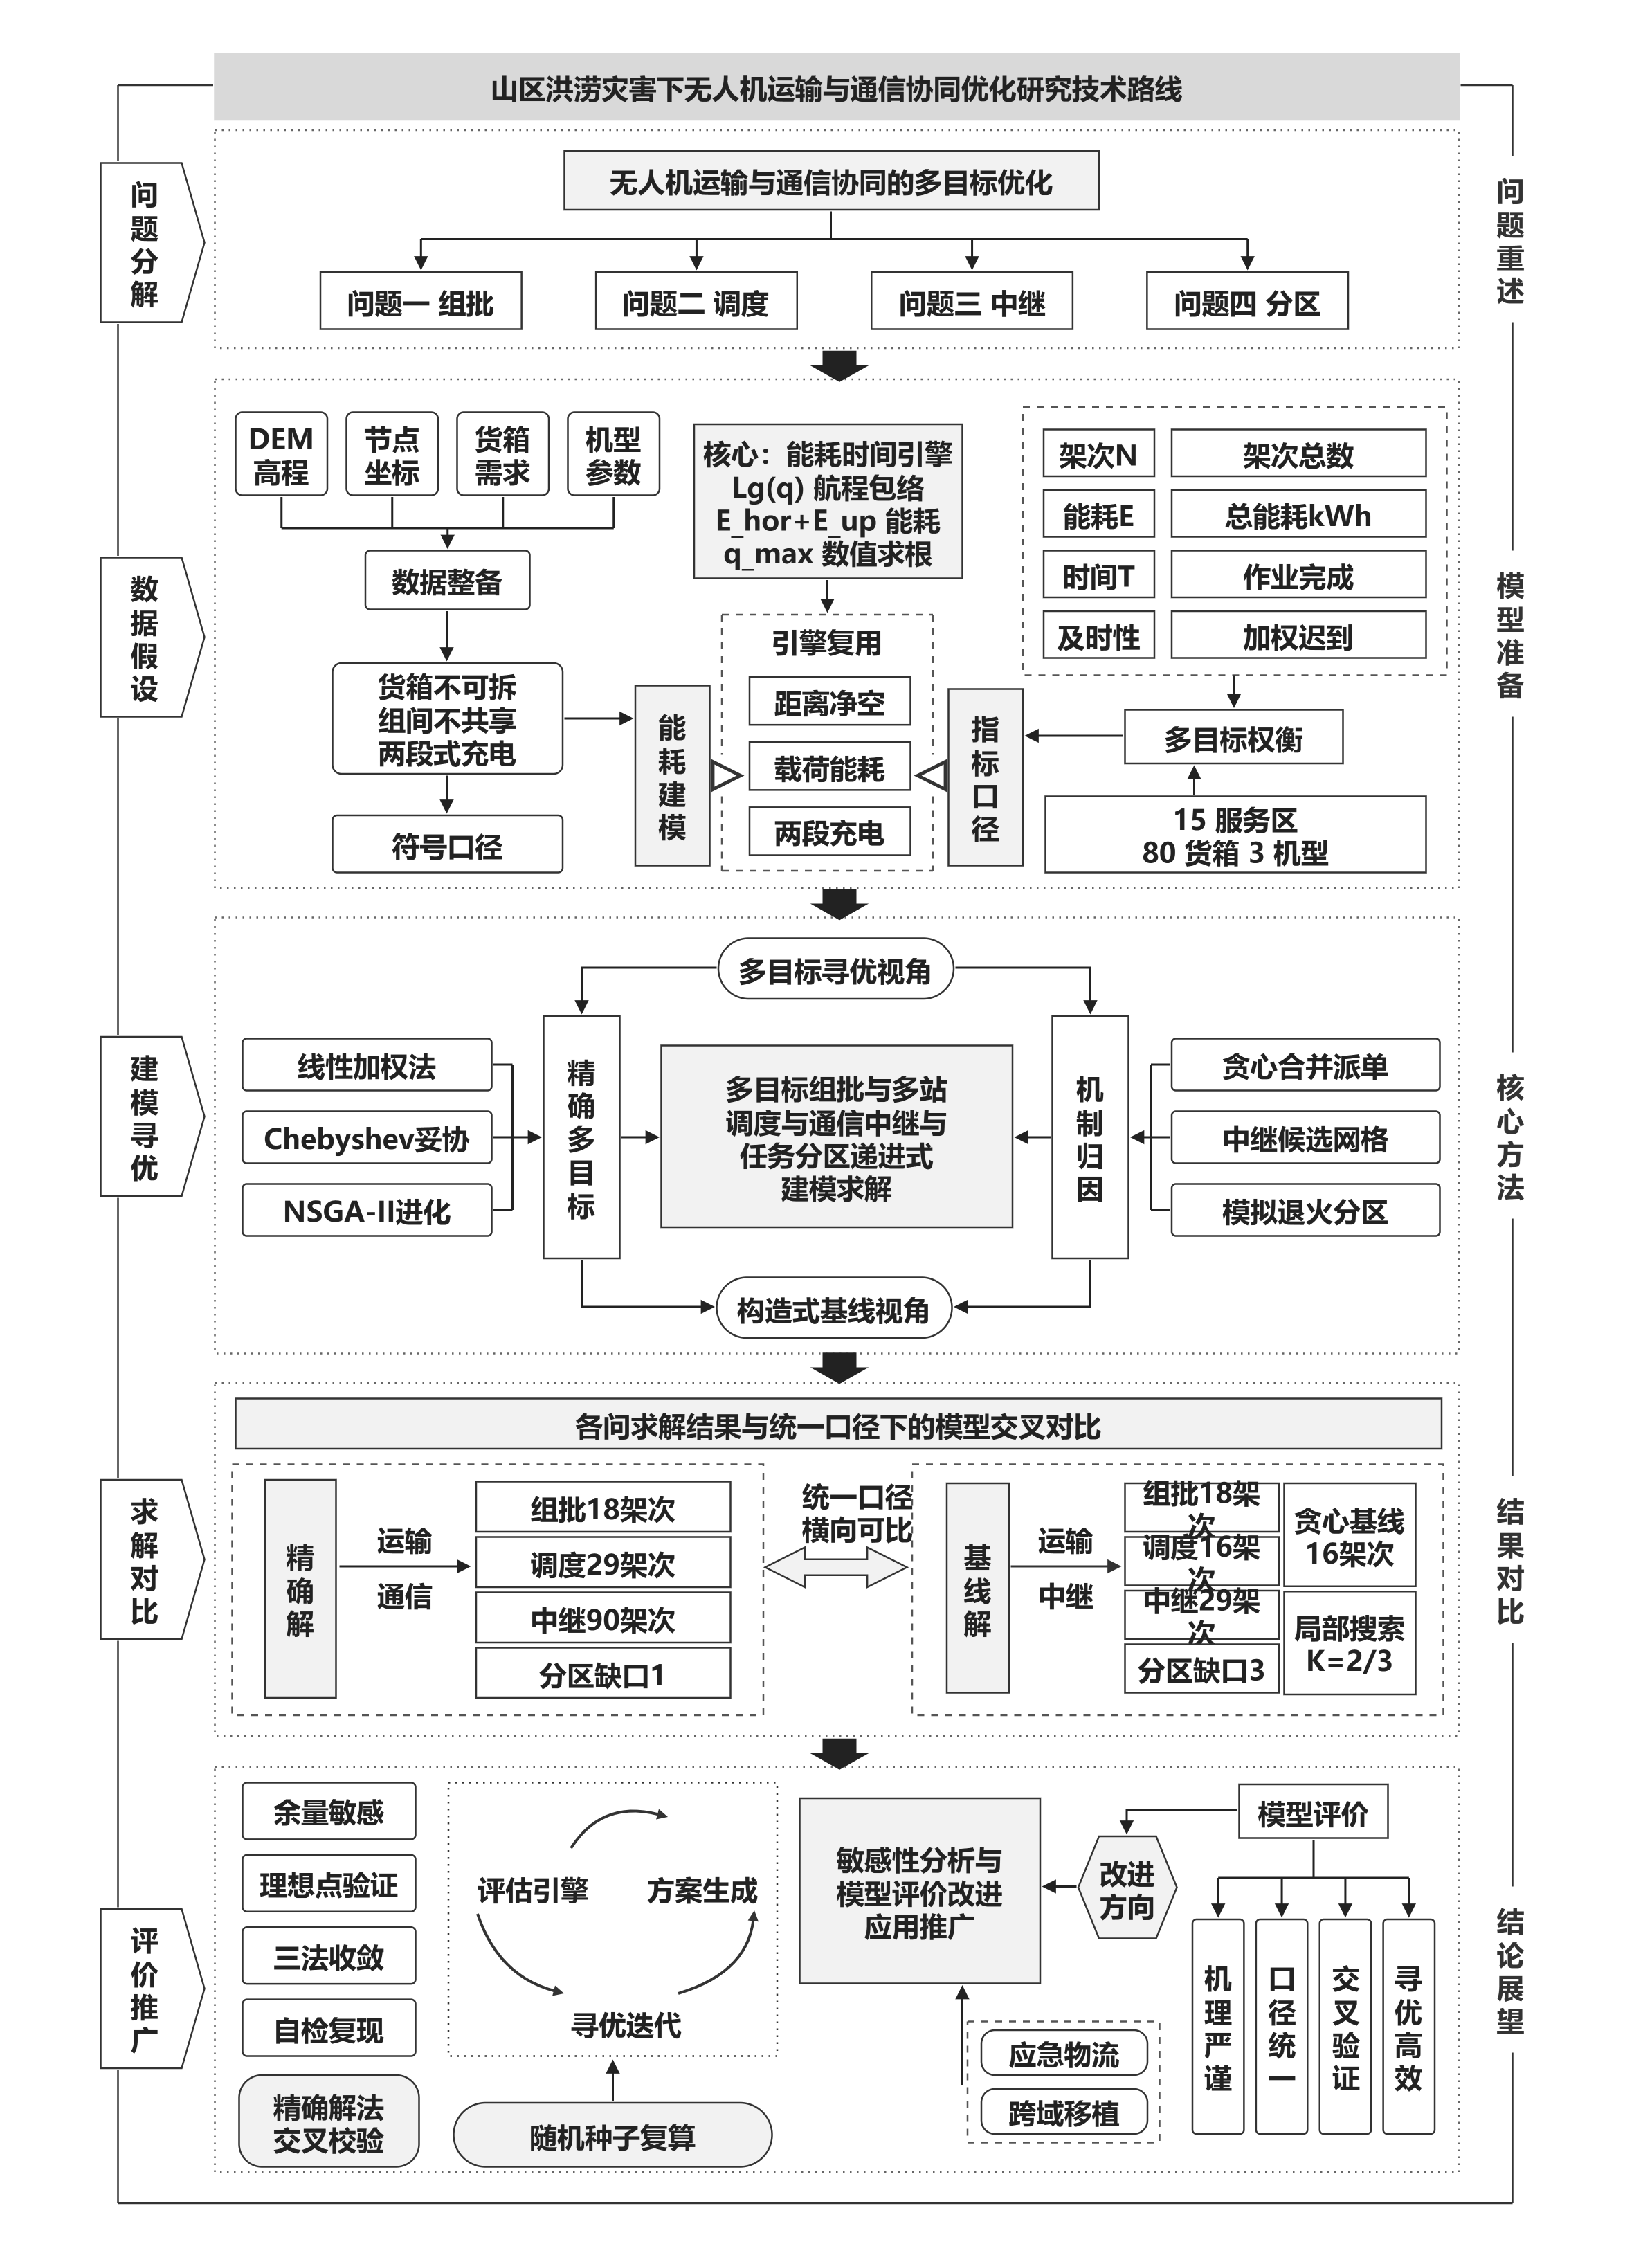
\includegraphics[width=0.72\textwidth]{figures/00_技术路线图.png}
\caption{全文技术路线图}
\label{fig:roadmap}
\end{figure}

\subsection{问题一的分析}

问题一的核心是"能力评估 + 组合优化"。输入为节点坐标、30\,m DEM、机型参数与货箱清单，输出为 45 组最大安全载荷 $q_{\max}(g,i)$ 与组批方案。

\textbf{最大安全载荷}是一个约束可行性问题而非优化问题：给定机型 $g$ 与服务区 $i$ 的往返航段几何，$q_{\max}$ 是使"去程（载 $q$）+ 返程（空载）"总能耗恰好等于返航能量上限 $(1-\rho)E^{\rm use}_g$ 的载荷。由于水平能耗模型随载荷单调递增，可用数值求根直接求解。

\textbf{货箱组批}是一个带质量/体积/能量三约束的装箱与集合划分问题。由于"每箱只装一次、同区组批、架次仅服务单区"，可将其建模为 0-1 集合划分（Set Partitioning）：先枚举每个服务区、每种机型下所有可行货箱子集（候选批次），再选择一组候选批次恰好覆盖全部货箱。

\textbf{多目标优化}需要同时权衡架次数 $N$、总能耗 $E$、累计作业时间 $T$ 三个目标。三者量纲不同且相互制约，需采用多目标方法刻画 Pareto 前沿与折中解；本题货箱组批在 15 个服务区间相互独立，三个目标均为各区分量的简单加总，这一可分结构既允许"逐区求局部 Pareto 再用 Minkowski 和合并"的精确分解，也便于用多种方法互相验证。

\textbf{返航余量敏感性}源于余量 $\rho$ 直接进入能量上限，改变 $\rho$ 会改变 $q_{\max}$ 乃至组批可行性，需量化其影响。

\subsection{问题二的分析}

问题二将"单点往返"扩展为"多点串行 + 资源调度"，是典型的多站车辆路径问题（Vehicle Routing Problem，VRP）与资源受限项目调度问题的耦合\cite{ref_dorling}。决策变量新增：多站路线的停靠顺序、每个架次的执行无人机与共享电池、各架次开始时刻。

难度在于：(1) 多站路线逐腿卸货后载荷单调下降，而水平能耗模型是载荷的凸函数，故能耗与停靠顺序相关，需对可行排列精确比较；(2) 8 架实体机 + 共享电池池 + 两阶段非线性充电构成离散事件资源调度，需保证资源区间不重叠；(3) 医疗/首批货箱带硬时限，需与软目标（及时性）分离处理。

考虑到问题规模（80 箱、15 区、3 机型）与强耦合约束，本文采用两种互补方法：其一为 NSGA-II 全局多目标进化求解（主方案，追求硬约束严格可行），其二为"贪心多站合并 + 派单规则扫描"的构造式方法（对比方法，可解释、节能）。二者分别对应"严格可行"与"少架次节能"两种取舍，可交叉讨论，并以严格可行方案作为问题三的承接基准。

\subsection{问题三的分析}

问题三在运输维度上叠加通信保障维度，形成运输无人机与中继无人机的联合调度。通信侧需判定每个时刻运输无人机与固定网关 G01 的链路可用性（直连或经中继单跳），链路可行性由自由空间损耗、DEM 地形遮挡与双向链路预算共同决定\cite{ref_itu,ref_zeng}。

关键难点在于：(1) 运输无人机全程连续通信，需按爬升/巡航/下降相位逐点判定遮挡；(2) 中继悬停位置与高度需在 DEM 覆盖范围内离散化搜索；(3) 中继无人机（2 架）与能源组件（6 个）构成独立资源池，与运输资源联合排程。本文主方案承接问题二贪心路线，进行中继候选网格枚举与集合覆盖分配；对比方案用 NSGA-II 对"路线 + 中继"联合优化，以量化通信保障带来的能耗与架次代价。

\subsection{问题四的分析}

问题四是一个"带 must-link 约束的集合划分 + 资源核算"问题。由于同一运输架次涉及的服务区必须同组，可先用并查集将 15 个服务区收缩为若干原子任务块；再对任务块做 K 组无标签分区，并对每组独立核算运输机、共享电池、中继机与中继能源组件的峰值并发需求（各组资源不共享）。

评价维度为资源缺口（gap）、资源配置总规模、组间工作量均衡系数、资源冗余四项。问题规模（收缩后 13 个任务块）允许完全枚举精确求解，故本文以完全枚举为主方案、保证分区全局最优；同时用负载均衡初始化 + 模拟退火局部搜索作为可扩展的对比方法，验证其在更大规模下的适用性，并与精确解对照以量化启发式与全局最优之间的差距。二者构成"精确最优"与"可扩展近似"的方法对。

\subsection{技术路线图}

全文技术路线如图~\ref{fig:roadmap} 所示，五条带分别对应破题分解、模型准备、核心方法、结果对比与评价推广，四问方法沿第三带横向展开、结果沿第四带统一口径对比。

\subsection{研究框架与创新点}

本文将四个子问题抽象为一条"能力评估 $\to$ 组批 $\to$ 调度 $\to$ 通信协同 $\to$ 分区配置"的递进式建模链，其核心是一个被四问共用的\textbf{公共物理引擎}与四层\textbf{逐问叠加的决策结构}：

\begin{enumerate}
    \item \textbf{公共物理引擎}：由 DEM 地形净空采样、航程包络反推水平能耗、重力势能爬升能耗、两阶段充电模型与作业时间模型共同构成，为问题一至问题四提供统一的能耗/时间/资源口径，保证各问结果可直接横向比较与逐问继承。
    \item \textbf{问题一（能力层）}：以"约束可行性求根 + 集合划分"评估单机能力并完成组批，输出 $q_{\max}$ 与组批方案，作为后续各问的输入。
    \item \textbf{问题二（调度层）}：叠加多站路线、实体机队、共享电池池与硬时限，形成"组批—路线—派单—资源排程"四层耦合的多目标调度。
    \item \textbf{问题三（通信层）}：在运输维度上叠加通信保障，引入地形遮挡判定、双向链路预算与中继悬停网格，形成运输与中继联合调度。
    \item \textbf{问题四（配置层）}：固定既有调度关系，仅做任务分区与资源峰值核算，评估"分组独立执行"对资源配置的影响。
\end{enumerate}

主要创新点有三：其一，针对规格表仅给航程字段而缺巡航功率的困难，提出"等效航程包络反推水平能耗"的建模口径，将离散的航程点扩展为随载荷连续变化的能耗函数；其二，利用组批决策在服务区间相互独立的可分结构，将多目标组批分解为"逐区局部 Pareto + Minkowski 和合并"，在保证全局前沿正确性的同时避免了组合爆炸；其三，在每问均构造"精确/最优方法 + 启发式/可扩展方法"的方法对（MILP 与 NSGA-II、完全枚举与模拟退火），用交叉验证而非单一方法支撑结论，显著增强了结果的正确性与可信度。
